\section{Le sens du Mouvement}
\subsection{Perception}
\begin{frame}{Perception}
\begin{multicols}{2}
\begin{itemize}
\item Perception du déplacement du corps dans l'espace
\item Système proprioceptif
\begin{itemize}
\item Système vestibulaire
\item Sens haptique
\end{itemize}
\end{itemize}
\begin{figure}
\centering
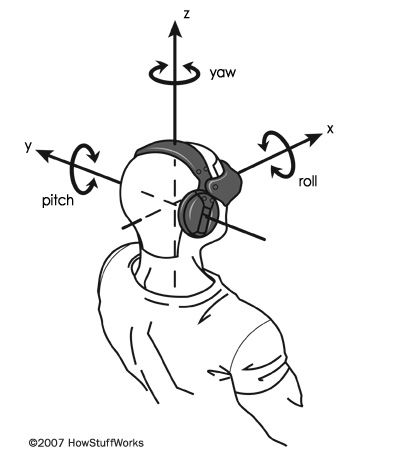
\includegraphics[width=5cm]{images/dof}
\end{figure}
\end{multicols}
\end{frame}

{
\setbeamertemplate{frame footer}{\copyright nasa.gov}
\begin{frame}{Perception - Système Vestibulaire}
\begin{itemize}
\item 3 canaux semi-circulaires $\rightarrow$ vitesse angulaire
\item 2 organes otolithiques $\rightarrow$ accélération linéaire
\begin{itemize}
\item Saccule
\item Utricule
\end{itemize}
\end{itemize}
\begin{figure}
\centering
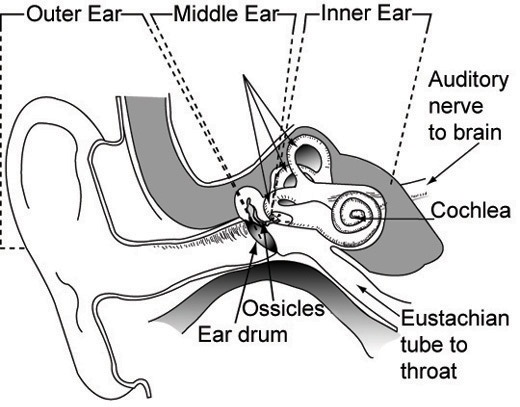
\includegraphics[width=5cm]{images/innerear}
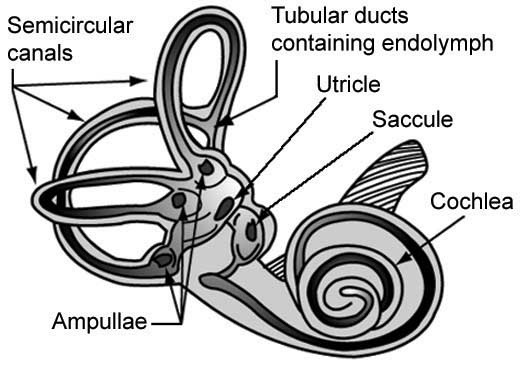
\includegraphics[width=5.6cm]{images/vestibular}
\end{figure}
\end{frame}
}

\subsection{Illusions de mouvement}
\begin{frame}{Illusions de mouvement}
\begin{multicols}{2}
\begin{itemize}
\item Organes otolithiques sont sensibles à la gravité
\end{itemize}
\begin{figure}
\centering
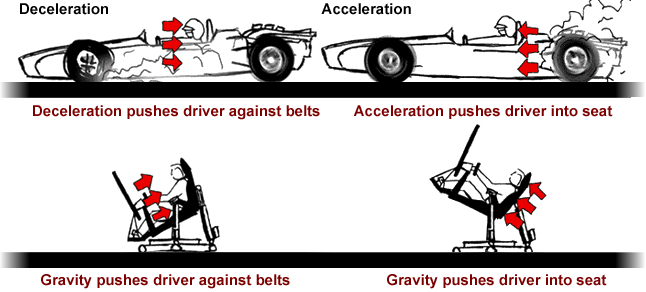
\includegraphics[width=5cm]{images/simulateurMovement}
\caption{\copyright force-dynamics.com}
\end{figure}
\begin{figure}
\centering
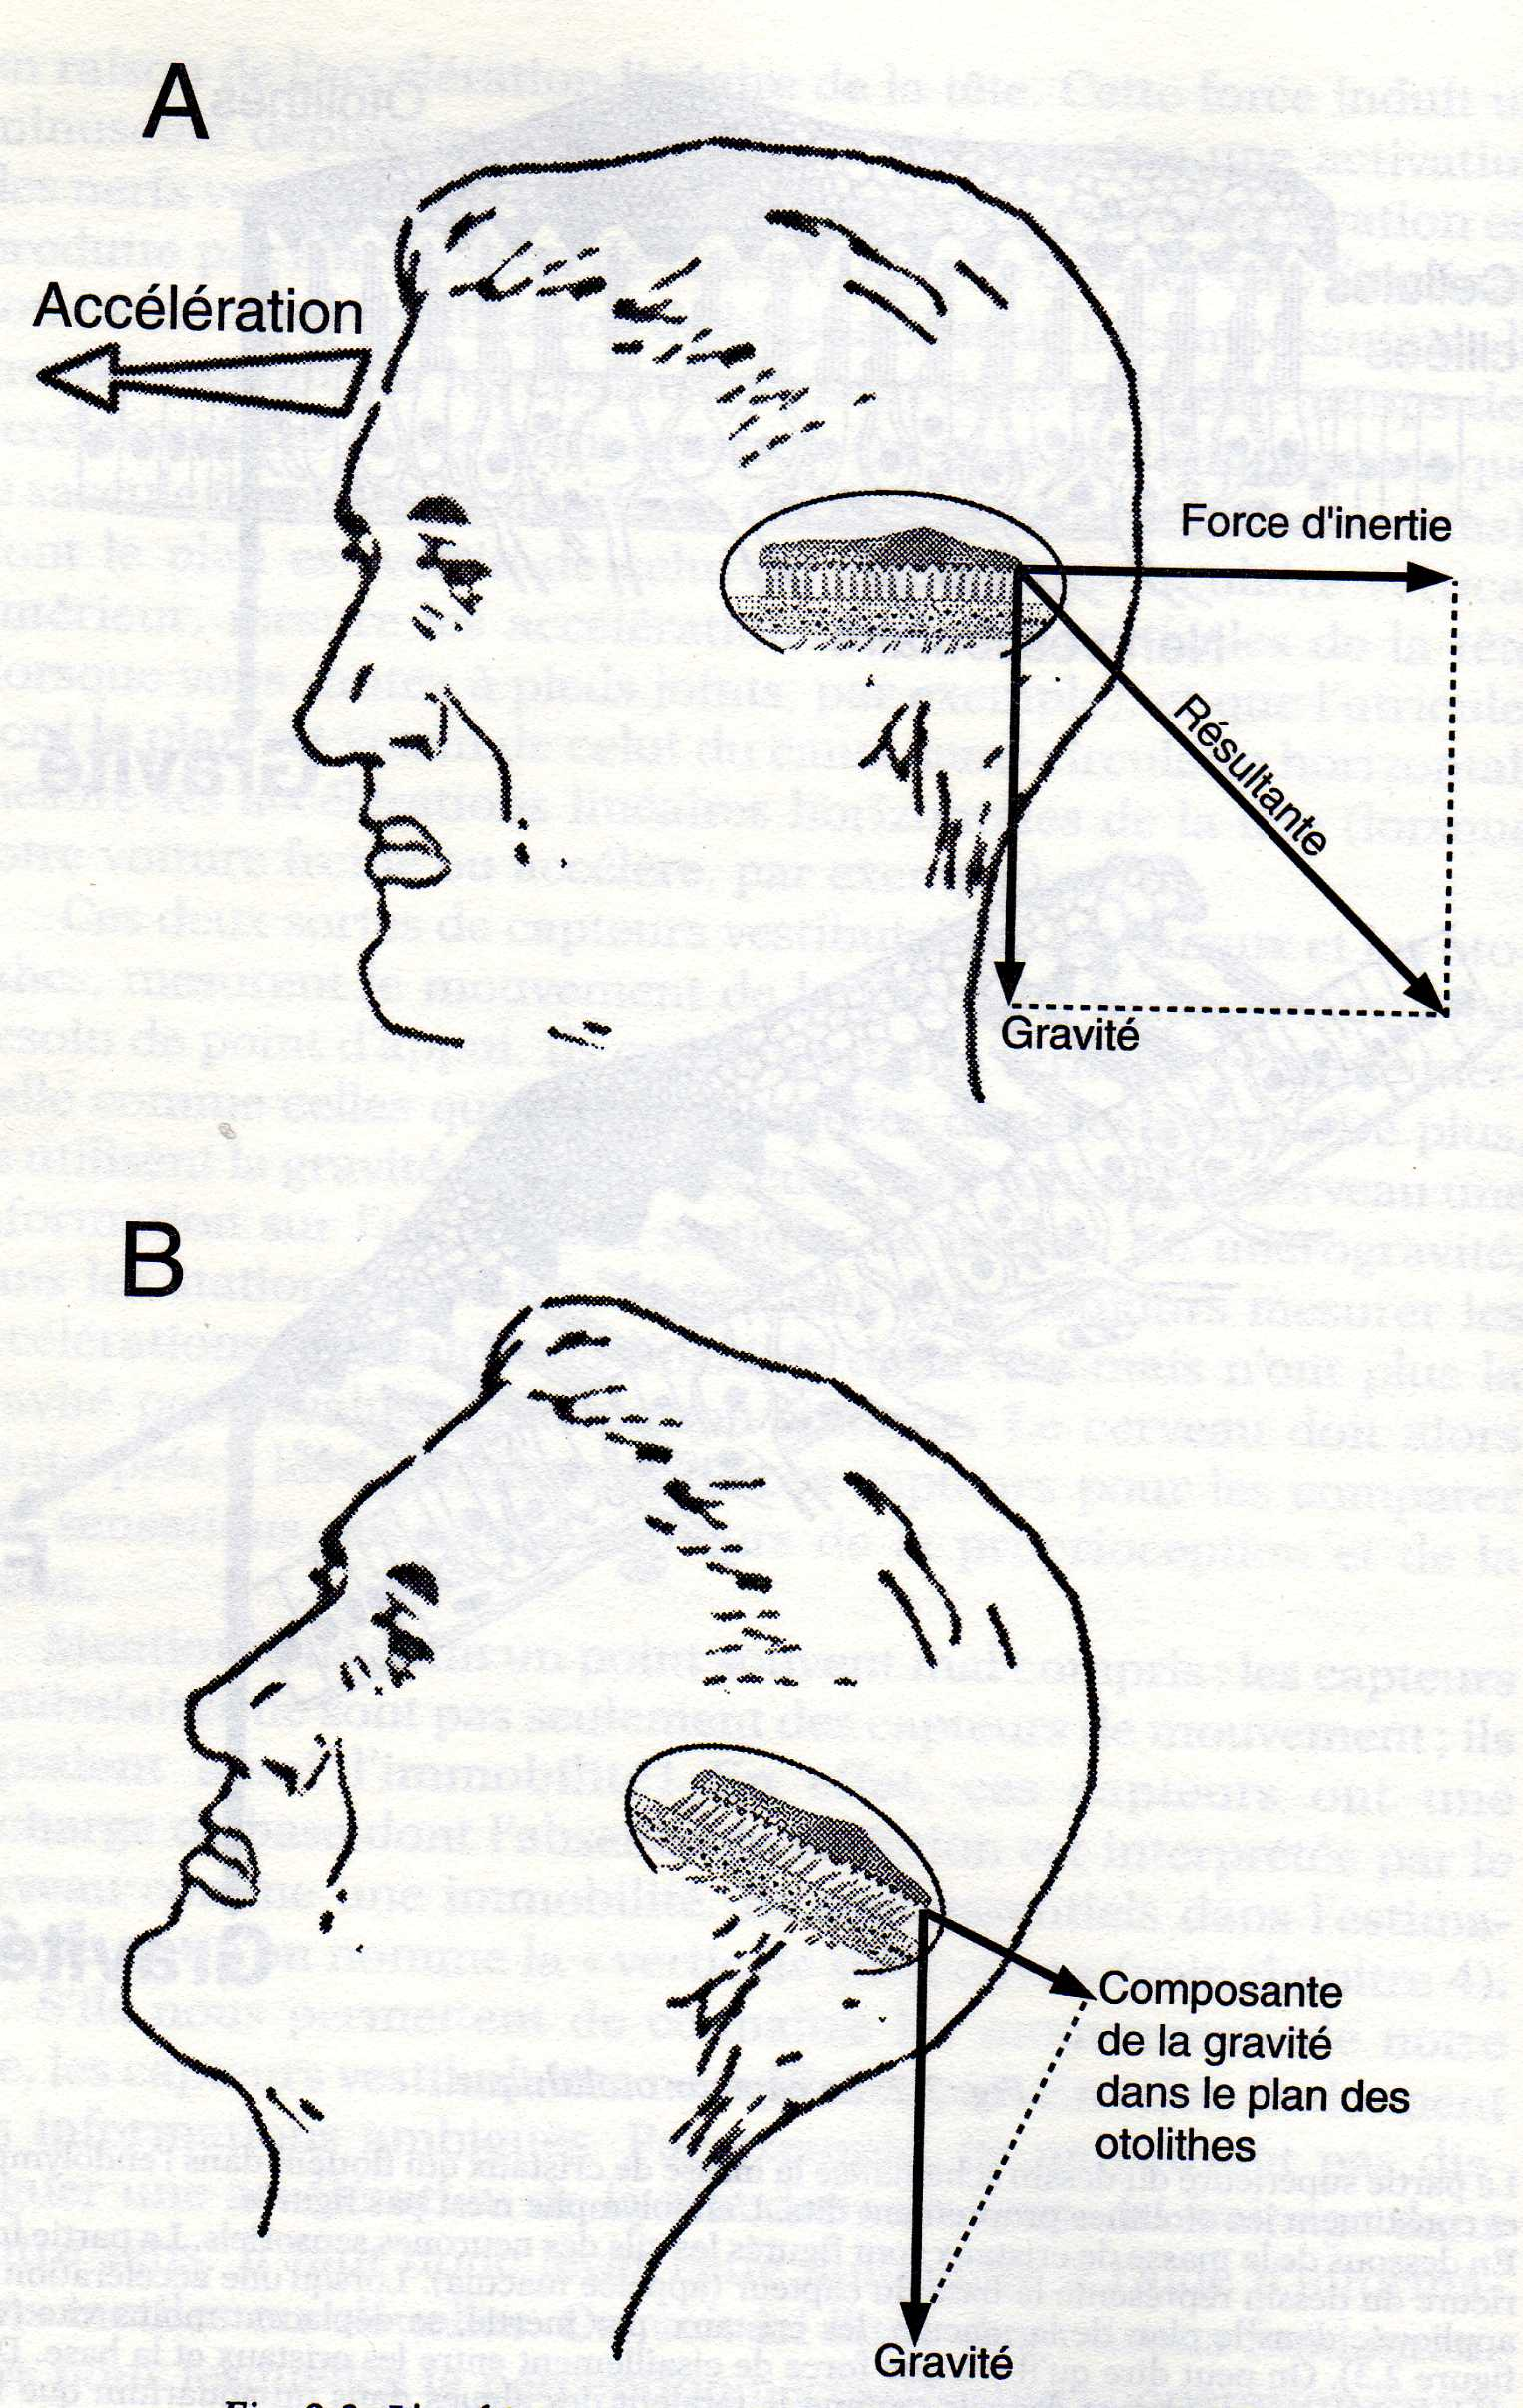
\includegraphics[width=4cm]{images/Berthoz001}
\caption{\cite{Berthoz1997}}
\end{figure}
\end{multicols}
\end{frame}

\begin{frame}{Illusions de mouvement}

\begin{itemize}
\item Vection : illusion de mouvement propre
\item "Illusion du train"
\item Provoquée part le système visuel
\end{itemize}
\begin{multicols}{2}
\begin{figure}
\centering
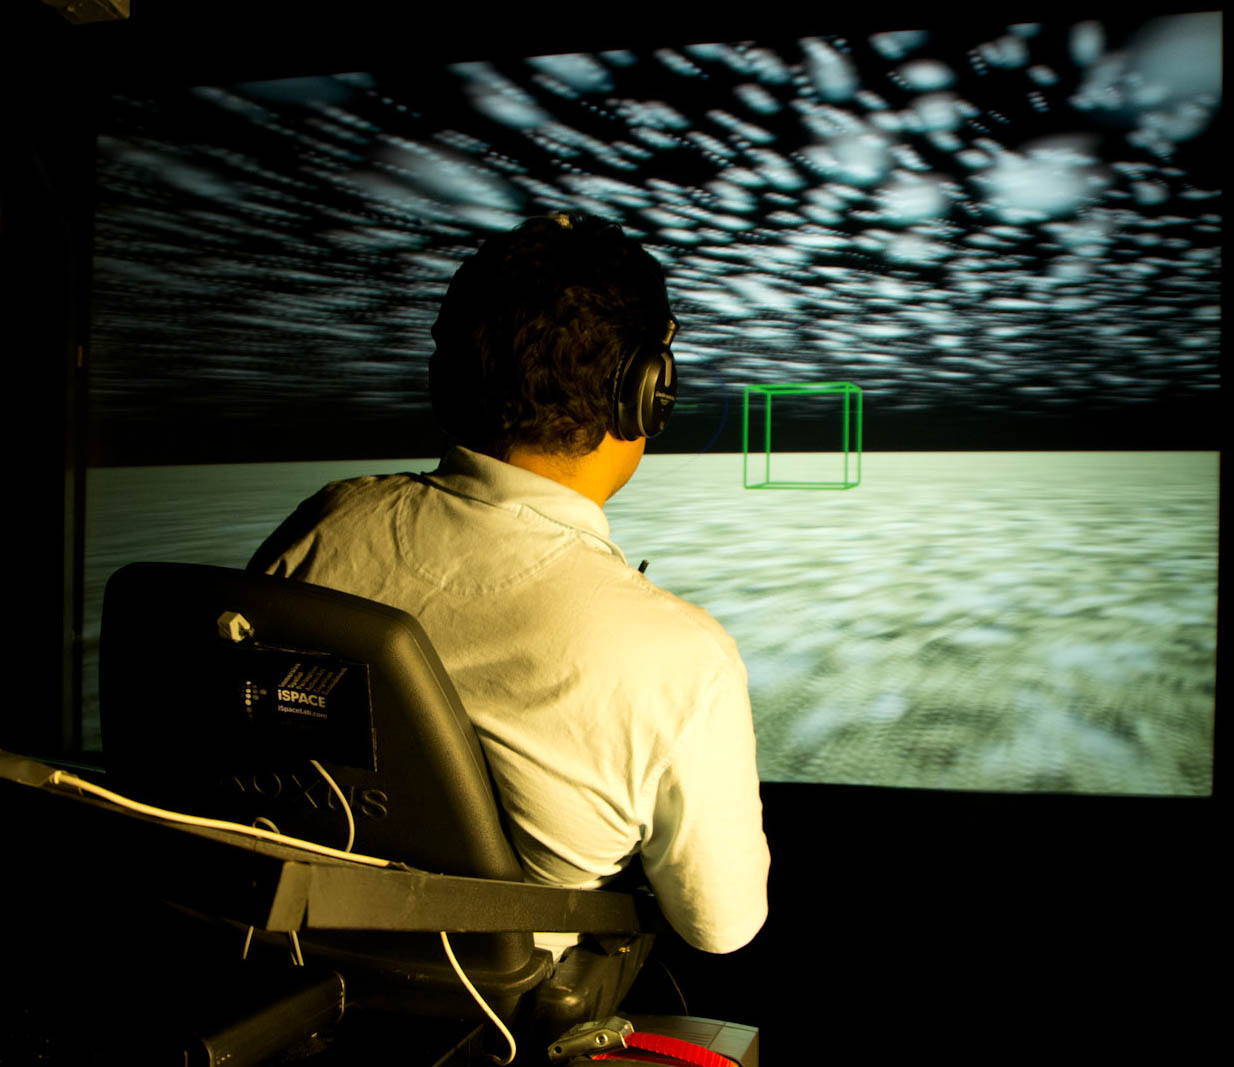
\includegraphics[width=5cm]{images/opticflow}
\caption{\cite{Riecke2005}}
\end{figure}
\begin{figure}
\centering
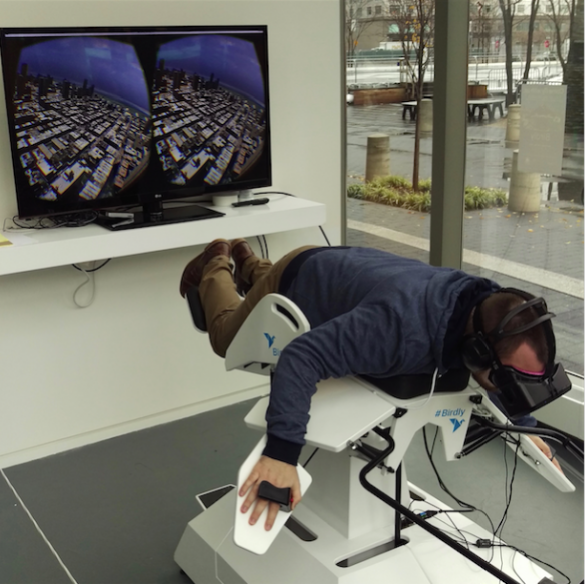
\includegraphics[width=4.3cm]{images/birdly}
\caption{\copyright Birdly - somniacs.co}
\end{figure}
\end{multicols}
\end{frame}

\subsection{Simulateur de mouvements}
\begin{frame}{Simulateur de mouvement}
\begin{itemize}
\item Basé sur la plateforme de Stewart (hexapode)
\item 6 degrés de liberté
\end{itemize}
\begin{multicols}{2}
\begin{figure}
\centering
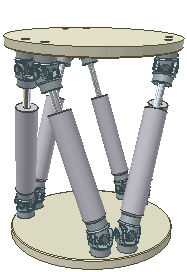
\includegraphics[width=3cm]{images/Hexapod}
\caption{\copyright Wikipedia.org}
\end{figure}
\begin{figure}
\centering
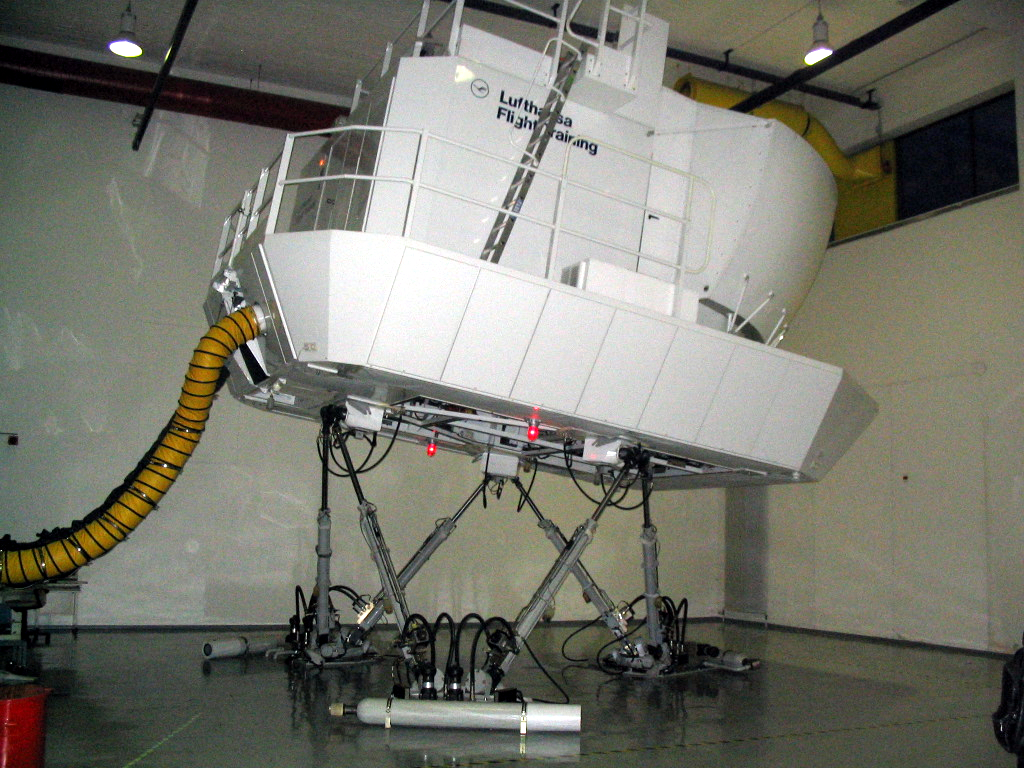
\includegraphics[width=5cm]{images/Simulator-flight}
\caption{\copyright Wikipedia.org}
\end{figure}
\end{multicols}
\end{frame}

{
\setbeamertemplate{frame footer}{\copyright d-box.com}
\begin{frame}{Simulateur de mouvement}
\begin{itemize}
\item Version simplifiée à 3 degrés de liberté
\item Utilisée pour les "cinémas 4D"
\end{itemize}
%\begin{multicols}{2}
\begin{figure}
\centering
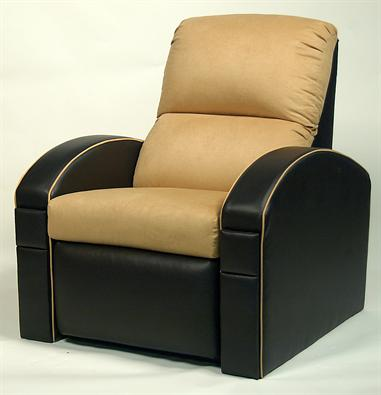
\includegraphics[height=4cm]{images/dbox1}
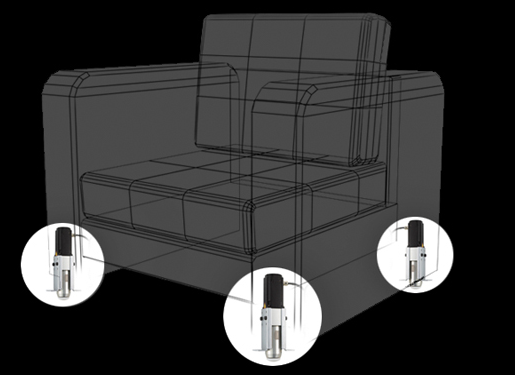
\includegraphics[height=4cm]{images/dbox}
\end{figure}
%\end{multicols}
\end{frame}
}

{
\setbeamertemplate{frame footer}{\cite{nehaoua2008design}}
\begin{frame}{Rendu de mouvement - Motion Platform}
\begin{itemize}
\item Washout Filter
\begin{itemize}
\item in: accélération linéraires et vitesse angulaires
\item out: position et orientation de la plate-forme
\item rate limit: $3^\circ/s$
\end{itemize}
\end{itemize}
\begin{figure}
\centering
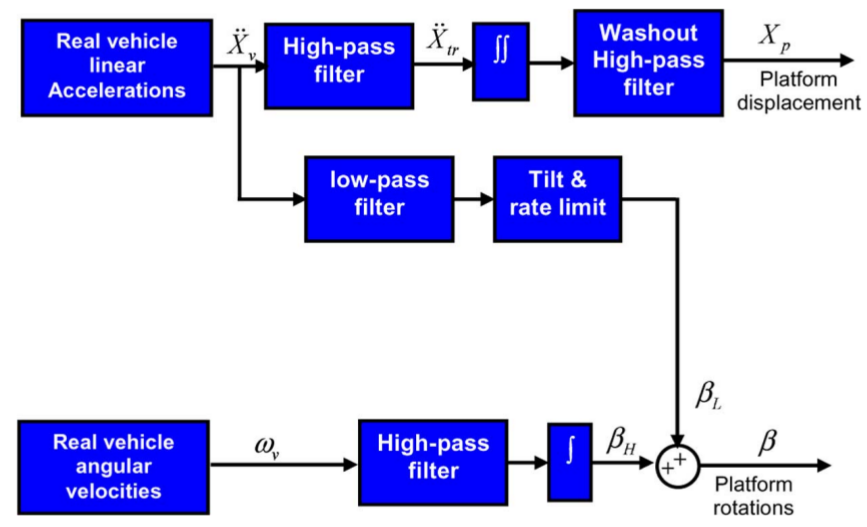
\includegraphics[width=8cm]{images/washout_filter}
\end{figure}
\end{frame}
}

\subsection{Autres simulateurs}

{
\setbeamertemplate{frame footer}{\cite{Maeda2005}}
\begin{frame}{Autres simulateurs}
\begin{itemize}
\item Stimulation galvanique vestibulaire
\item Électrodes derrière les oreilles
\item 1 degré de liberté
\end{itemize}
\begin{figure}
\centering
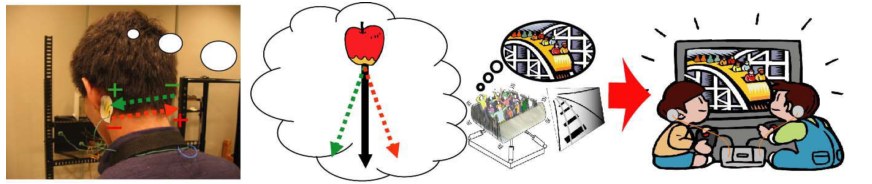
\includegraphics[width=10cm]{images/gvs_RV}
\end{figure}
\end{frame}

\begin{frame}{Autres simulateurs}
\begin{figure}
\href{run:videos/GVS.mp4}{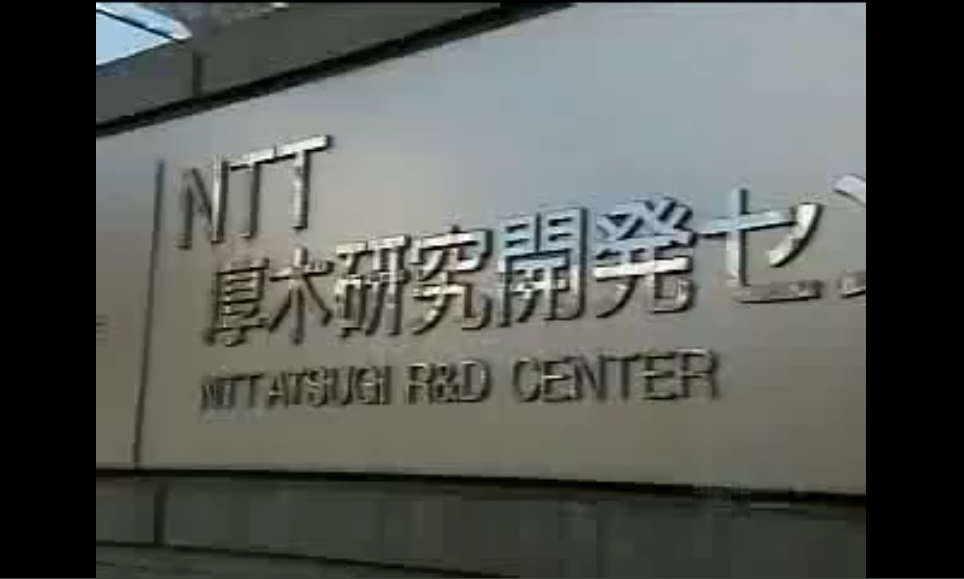
\includegraphics[width=\linewidth]{images/gvs}}
\end{figure}

\end{frame}
}

{
\setbeamertemplate{frame footer}{\cite{costes2022kinesthetic}}
\begin{frame}{Autres simulateurs}
\begin{figure}
\href{run:videos/khmd.mp4}{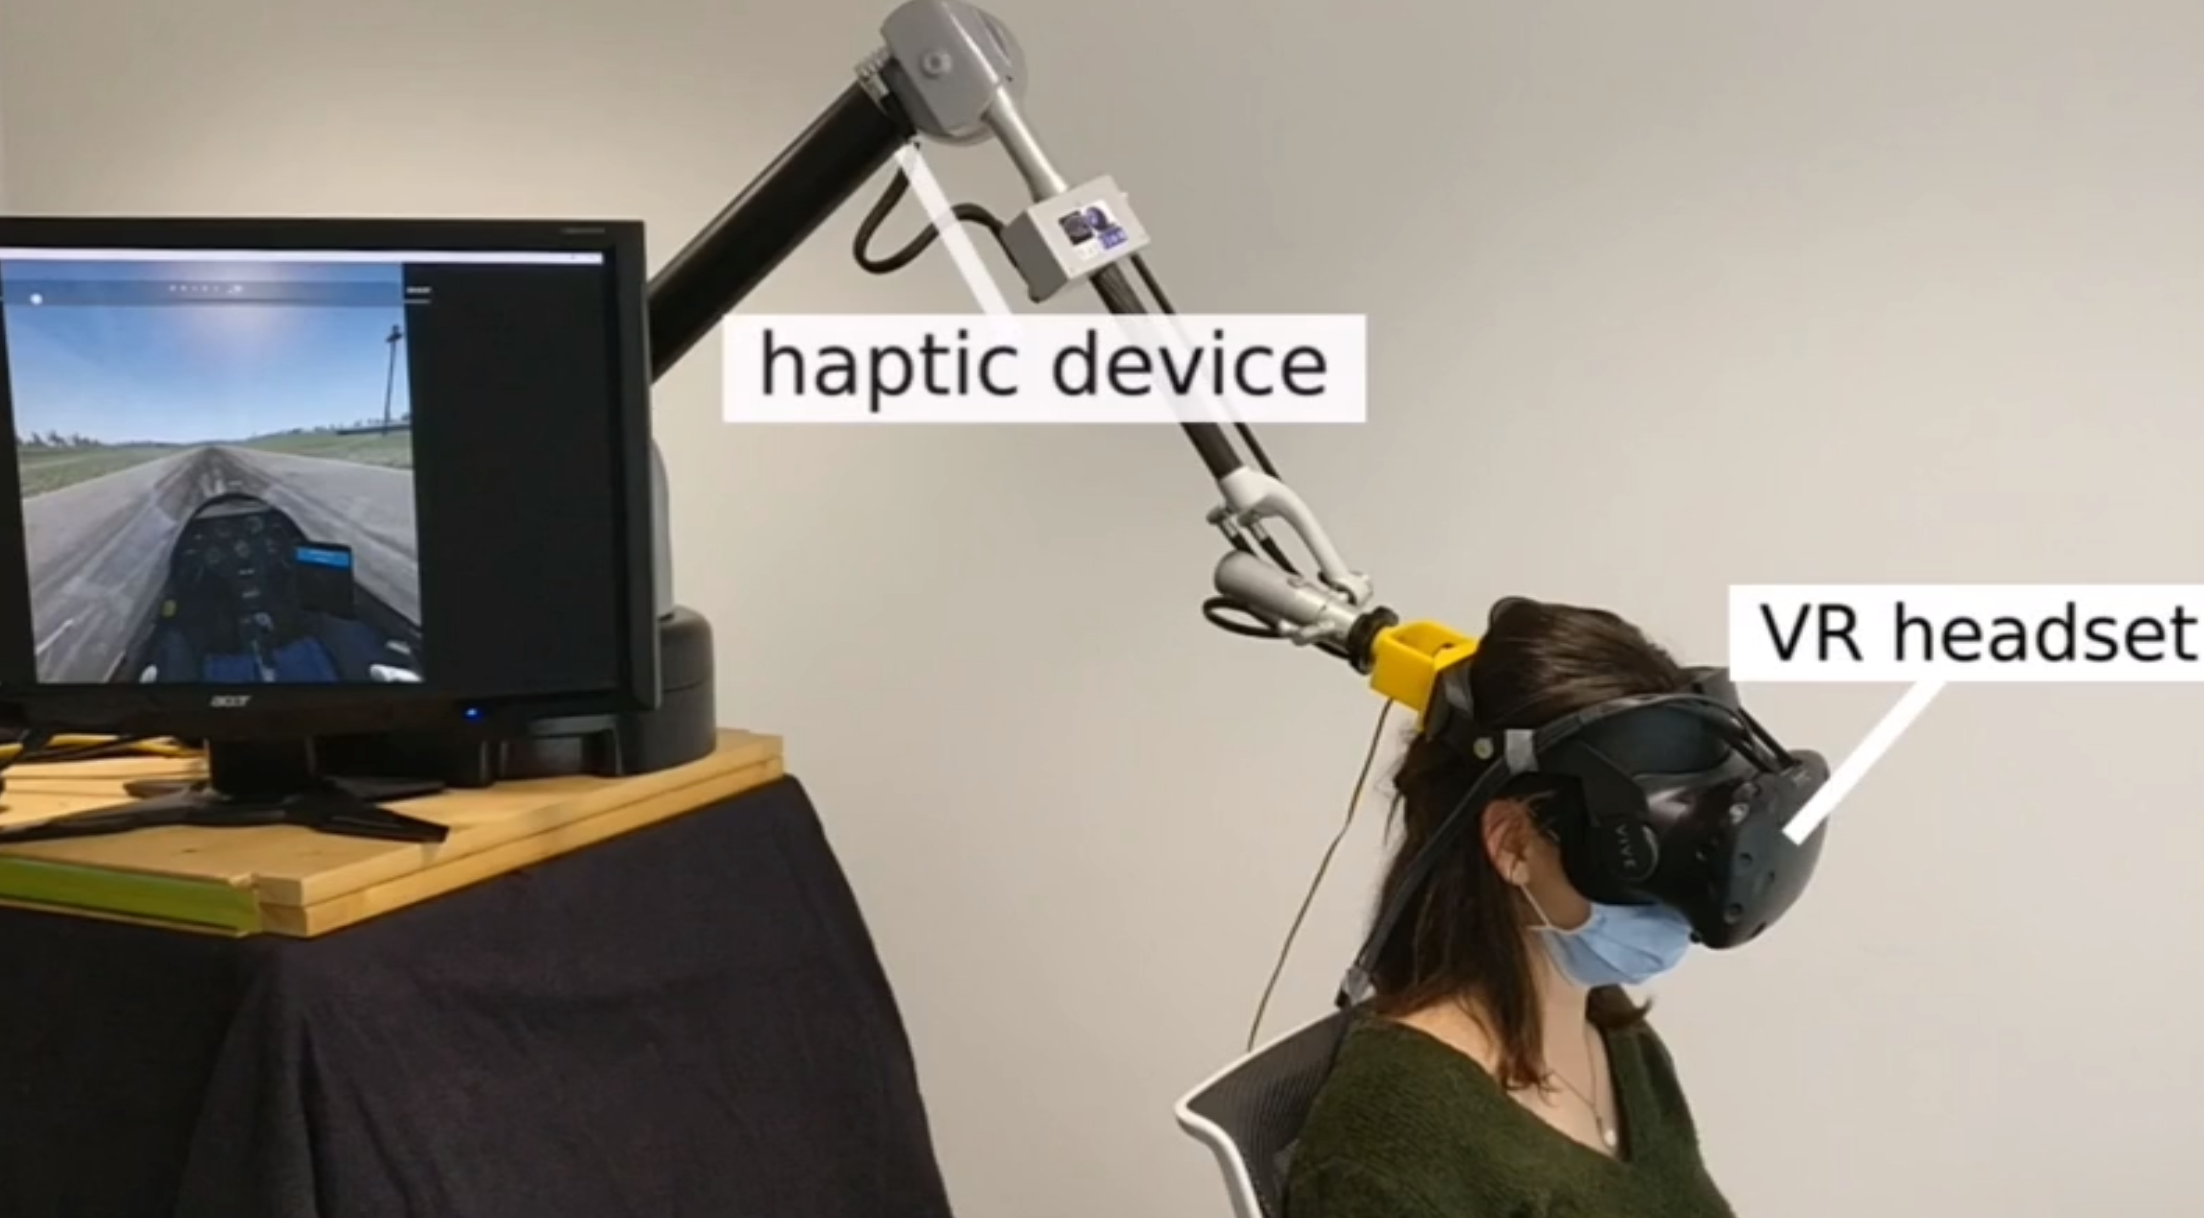
\includegraphics[width=\linewidth]{images/khmd}}
\end{figure}

\end{frame}
}

{
\setbeamertemplate{frame footer}{\cite{Danieau2012b}}
\begin{frame}{Autres simulateurs}
\begin{itemize}
\item HapSeat
\item 6 degrés de liberté
\item Retours de force locaux (tête et mains)
\end{itemize}
\begin{figure}
\centering
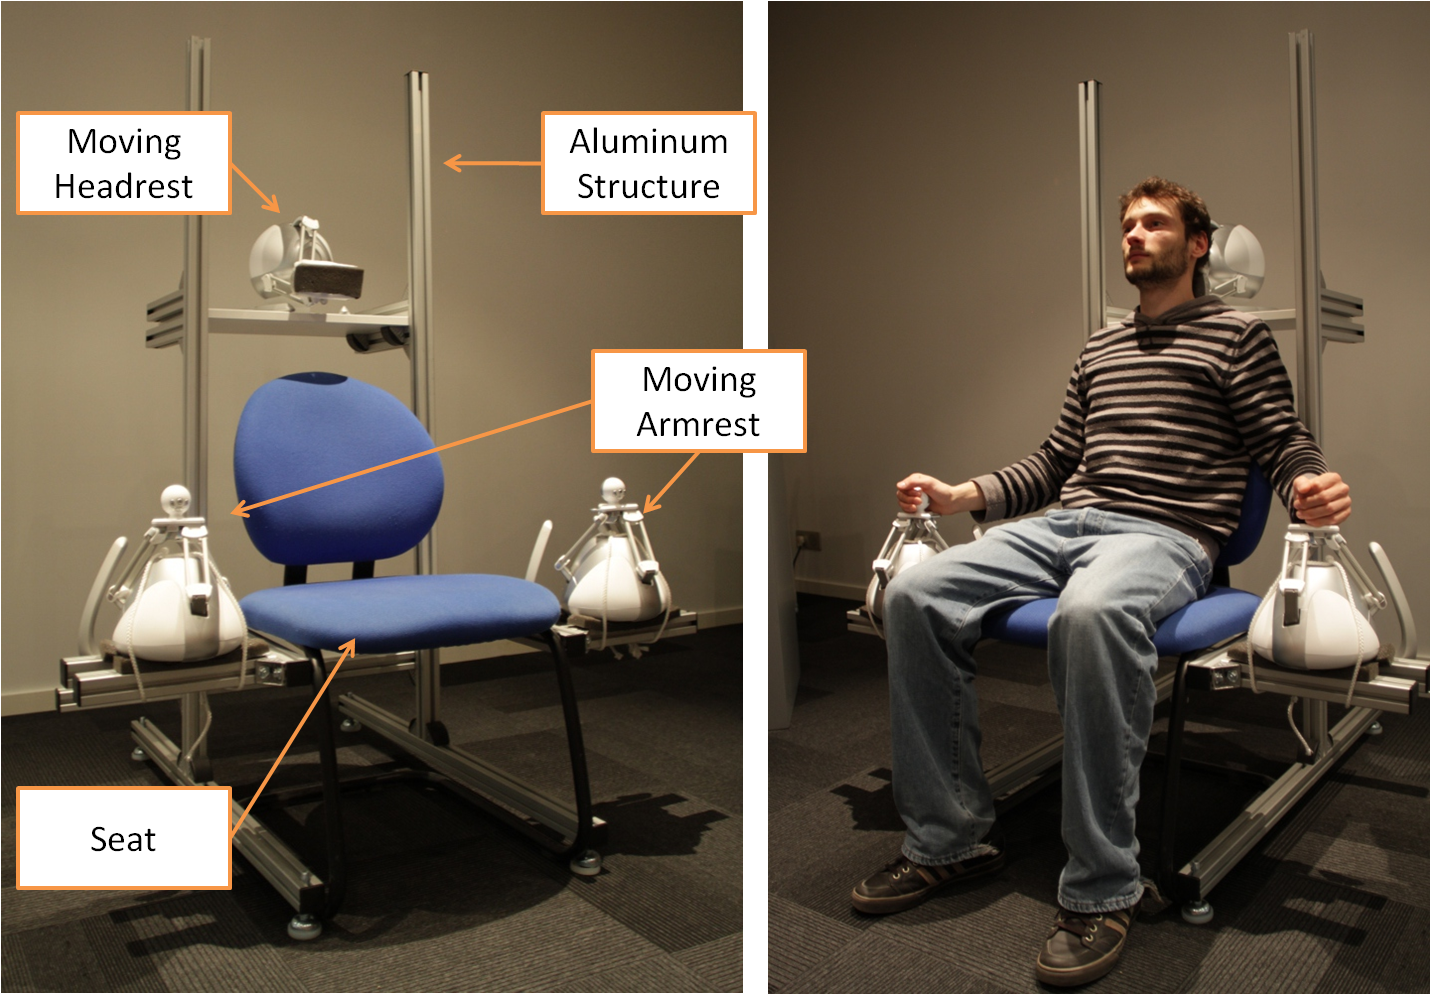
\includegraphics[width=8cm]{images/prototype}
\end{figure}
\end{frame}

\begin{frame}
\begin{figure}
\href{run:videos/HapSeat.avi}{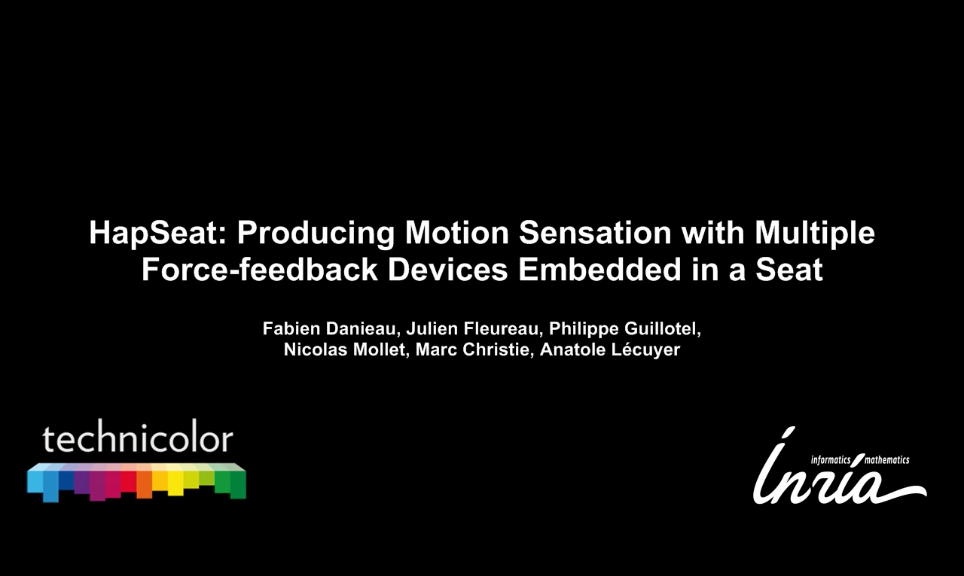
\includegraphics[width=\linewidth]{images/hapseat}}
\end{figure}

\end{frame}
}

{
\setbeamertemplate{frame footer}{\cite{Danieau2012b}}
\begin{frame}{Rendu de mouvement - HapSeat}
\begin{itemize}
\item Mouvement décrit par accélération linéraires ($a^t = [x_c,y_c,z_c]^t$) et vitesses angulaires ($w^t = [\phi_c, \theta_c, \psi_c]^t$)
\item Capturé par centrale inertielle
%\item $C^t = [x_c,y_c,z_c, \phi_c, \theta_c, \psi_c]^t$
\end{itemize}
\begin{figure}
\centering
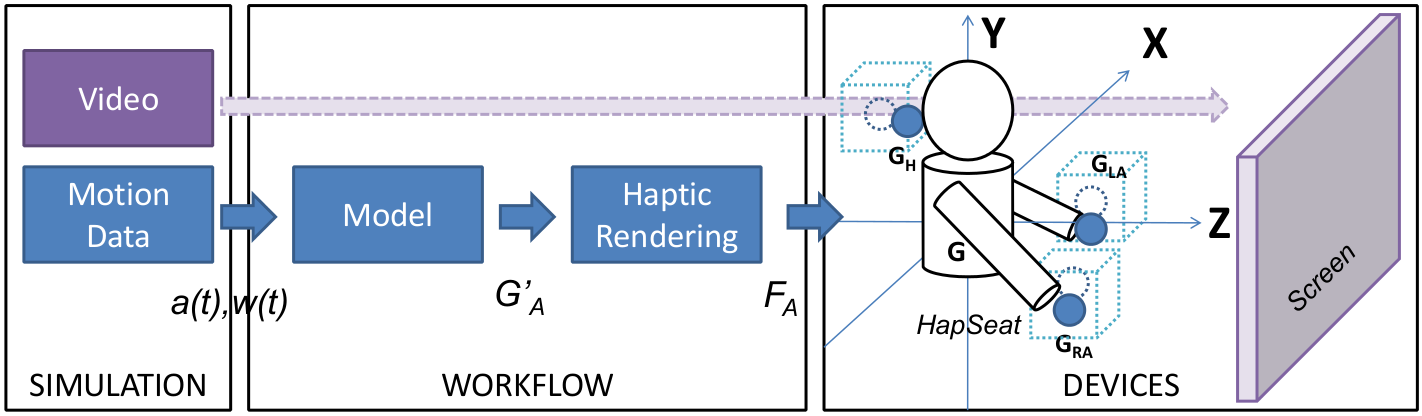
\includegraphics[width=\linewidth]{images/workflow}
\end{figure}
\end{frame}
}

\begin{frame}{Rendu de mouvement - HapSeat}
 \begin{equation}
 \overrightarrow{G_AG'_A} = f(\vec{T},\vec{R})
 \end{equation}
 avec
 \begin{equation}
f(\vec{T},\vec{R}) = \frac{\|\vec{T}\|\vec{T} + \|\vec{R}\|\vec{R}}{\|\vec{T}\| + \|\vec{R}\|}
\end{equation}
et
\begin{equation}
\vec{T} = \begin{bmatrix}
k_x & 0 & 0 \\
0 & k_y & 0 \\
0 & 0 & k_z
\end{bmatrix}
\begin{bmatrix}
x_c\\
y_c\\
z_c
\end{bmatrix} 
\label{eq:T}
\end{equation}
 
%\begin{equation}
%\begin{split}
%\vec{R} = (R_x(m_x \phi_c(t)) R_y(m_y \theta_c(t)) R_z(m_z \psi_c(t)) \\ 
% - I_3) \overrightarrow{GG_A})
%\end{split}
%\end{equation}

\begin{equation}
\vec{R} = (R_x(m_x \phi_c(t)) R_y(m_y \theta_c(t)) R_z(m_z \psi_c(t)) - I_3)\overrightarrow{GG_A})
\end{equation}

$k,m =$coefficients de réduction; $I_3 =$ matrice identité

\end{frame}

\begin{frame}{Rendu de mouvement - HapSeat}

\begin{equation}
\overrightarrow{GG'_A} = (R_x(m_x \phi_c(t)) R_y(m_y \theta_c(t)) R_z(m_z \psi_c(t))\overrightarrow{GG_A}
\end{equation}
i.e.:
\begin{subequations}
\begin{align}
\overrightarrow{G_AG'_A}& = \overrightarrow{GG'_A} - \overrightarrow{GG_A}\\
&=(R_x(m_x \phi_c(t)) R_y(m_y \theta_c(t)) R_z(m_z \psi_c(t))\overrightarrow{GG_A} - \overrightarrow{GG_A}\\
&=(R_x(m_x \phi_c(t)) R_y(m_y \theta_c(t)) R_z(m_z \psi_c(t))-I_3)\overrightarrow{GG_A}
\end{align}
\end{subequations}

\end{frame}
 
\begin{frame}{Rendu de mouvement - HapSeat}
\begin{multicols}{2}
\begin{itemize}
\item Novint Falcon = contrôle en impédance (force)
\item Modèle donne une position
\item Calcul de la force (modèle ressort-amortissement)
\item $F_A = k(G'_A - P_A) - d V_A$
\end{itemize}
\footnotesize{$k$ constante de ressort, $d$ constante d'amortissement}

\begin{figure}
\centering
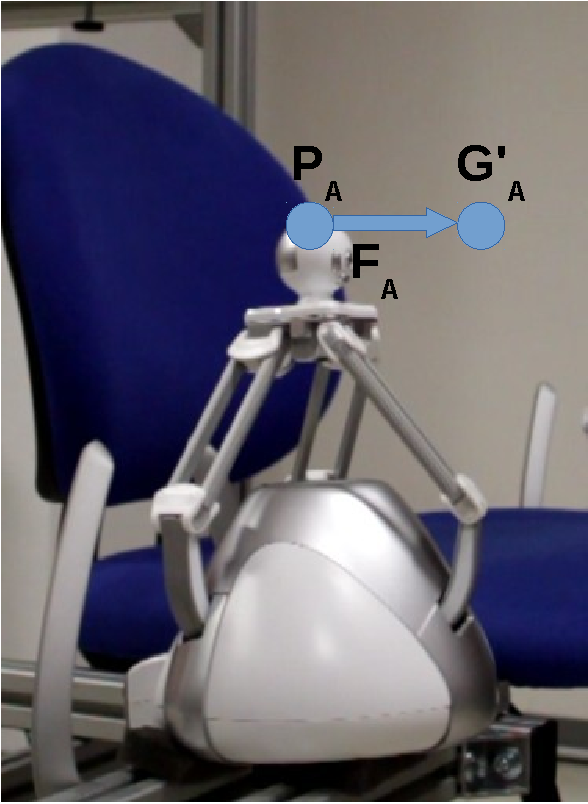
\includegraphics[width=5cm]{images/falcon}
\end{figure}


\end{multicols}
\end{frame}